\documentclass{article}

\usepackage{amsmath,amssymb,scalerel,amsthm}
\usepackage{derivative}
\usepackage{mathtools}
\usepackage{color}
\usepackage{tikz}


\title{Topology}
\author{Alessio Esposito}

\newtheorem{proposition}{Proposition}
\newtheorem{definition}{Definition}
\newtheorem{corollary}{Corollary}
\newtheorem{example}{Example}
\newtheorem{theorem}{Theorem}
\newtheorem{obs}{Observation}
\newtheorem{lemma}{Lemma}

\begin{document}
\maketitle
\begin{definition}
    let $X$ be a not empty set and $\mathcal{T}$ a collection of its subsets. $\mathcal{T}$ is said topology on $X$ if it has the following propeties:
    \begin{itemize}
        \item $\varnothing, X \in \mathcal{T}$
        \item the union of a whatever family of elements of $\mathcal{T}$ is in $\mathcal{T}$. In simbols: $\forall \{A_i \}_{i \in I}, \ A_i \in \mathcal{T}, \ \bigcup_{i \in I}A_i \in \mathcal{T}$  
        \item the intersection of elements of $\mathcal{T}$ is in $\mathcal{T}$: \ $\forall A_1, A_2 \in \mathcal{T}, \ A_1 \cap A_2 \in \mathcal{T} $ 
    \end{itemize}
Then $(X,\mathcal{T})$ its said to be topological space and $X$ is called support. 
\begin{example}
    Let $X = \mathbb{R}^2$ with the euclidean distance and $\forall c \in \mathbb{R}^2$ and $\forall r > 0$ the set $B_r(c) = \{ x \in \mathbb{R}^2 : d(x,c) < r \}$ its said open spherical neighbourhood of center $c$ and radius $r$.
    Let $\mathcal{T}$ be the totality of all the possible unions of open spherical neighbourhoods. $\mathcal{T}$ is a topology.

\end{example}
\end{definition}
\begin{definition}
    $(X_1, \mathcal{T}_1), \ (X_2, \mathcal{T}_2)$ topological spaces with $X_1 \cap X_2 = \varnothing.$ 
     \\ let $X = X_1 \cup X_2, \mathcal{T} = \{ A_1 \cup A_2 \ | \ A_i \in \mathcal{T}_i \}.$
\end{definition}
    \begin{lemma}
        $(X, \mathcal{T})$ is a topological space.
    \end{lemma}    
    \begin{proof}
        Lets verify the axioms.
        \begin{enumerate}
            \item $ \varnothing \in \mathcal{T}_1, \ \varnothing \in \mathcal{T}_2 \Rightarrow \varnothing = \varnothing \cup \varnothing \\ X_i \in \mathcal{T}_i \Rightarrow X = X_1 \cup X_2 \in \mathcal{T}$
            \item $\{A\}_{i\in I} \in \mathcal{T} \Rightarrow A_i = A_{1,i} \cup A_{2,i} \\ \bigcup_{i \in I}A_i = \bigcup_{i \in I}(A_{1,i} \cup A_{2,i}) = \bigcup_{i \in I}(A_{1,i}) \cup \bigcup_{i \in I}(A_{2,i}) \in \mathcal{T}_1 \cup \mathcal{T}_2$
            \item $ A, A' \in \mathcal{T} \Rightarrow A = A_1 \cup A_2, A' = A_1' \cup A_2' \\ A \cap A' = (A_1 \cup A_2) \cap (A_1' \cup A_2') = (A_1 \cap A_1') \cup (A_2 \cap A_2') \in \mathcal{T}  $ 
        \end{enumerate}

    \end{proof}
    \begin{definition}
        $\mathcal{T}$ is defined as a sum of Topologies $\mathcal{T}_1$ and $\mathcal{T}_2$. \\ We notice that $\forall A_i \in \mathcal{T}_i, \ A_i \cup \varnothing \in \mathcal{T}$ so $\mathcal{T}$ contains $\mathcal{T}_1$ and $\mathcal{T}_2.$  
    \end{definition}
        
    \begin{definition}
        $(X, \mathcal{T})$ topological space $\mathsf{Y} \subseteq X, \ \mathsf{Y} \neq \varnothing \\ \mathcal{T}_{/Y} = \{ A\cap \mathsf{Y} \ | \ A \in \mathcal{T} \}$ prove that $\mathcal{T}_{/Y}$ is a topology defined as Inducted topology on $Y$
    \end{definition}
    \begin{definition}
        $(X,\mathcal{T})$ topological space. $\mathcal{B} = \{ B_j\}_{j\in J}$ with $B_j \in \mathcal{T}$. $\mathcal{B}$ is said basis for the topology $\mathcal{T}$ if all open sets are union of elements of $\mathcal{B}$  
    \end{definition}
    \begin{lemma}
        Let $X \neq \varnothing$ and $\mathcal{B} \in \mathcal{P}(X)$. Let $A \subseteq X$ then the following affirmations are equivalent:
        \begin{itemize}
            \item[(a)] $A$ is union of elements of $\mathcal{B}$
            \item[(b)] $\forall x \in A \ \exists B \in \mathcal{B} : x\in B \subseteq A$ 
        \end{itemize}
        \begin{proof}
            \subsubsection*{(a) $\Rightarrow$ (b)}
                Let $x \in A = \bigcup_{i \in I}B_i$ with $B_i \in \mathcal{B}$. Therefore $\exists B_i: x\in B_i \subseteq A$ 
            \subsubsection*{(b) $\Rightarrow$ (a)}
                ($\subseteq$) \ $A = \bigcup_{i\in I} B_i \Rightarrow \forall x \in A \exists B_x : x\in B_x \Rightarrow A \subseteq \bigcup_{i\in I} B_i$. \\
                ($\supseteq$) \ $\forall x \in A \ \exists B_i \in \mathcal{B} : x\in B_i \subseteq A \Rightarrow A \subseteq \bigcup_{i_x\in I}B_{i_{x}}\subseteq A \Rightarrow A = \bigcup_{x\in A}B_x$
        \end{proof}
    \end{lemma}
    \begin{theorem}
        Let $X$ be a not empty set and $\mathcal{B} \in \mathcal{P}(X)$. $\mathcal{B}$ is a basis if:
        \begin{itemize}
            \item[$1.$] $X = \bigcup_{B\in \mathcal{B}}B$
            \item[$2.$] $\forall B_1, B_2 \in \mathcal{B}$ and $\forall x \in B_1 \cap B_2$ there exists $B_3 \in \mathcal{B} : x\in B_3 \subset B_1\cap B_2 $. 
        \end{itemize}
        \begin{proof}
            \subsubsection*{($\Rightarrow$)}
                Let $\mathcal{B}$ a basis such that every open set $A$ is union of elements of $\mathcal{B}$, in particular $X = \bigcup_{B\in \mathcal{B}}B$ moreover because $\mathcal{B} \subseteq \mathcal{T}$ we can say that $B_1,B_2 \in \mathcal{T}$ so is union of elements of $\mathcal{B}$. The last Lemma implies $\forall x \in B_1\cap B_2 \ \exists B_3 \in \mathcal{B}$ such that $x\in B_3 \subseteq B_1 \cap B_2$.
            \subsubsection*{($\Leftarrow$)}
                Let $\mathcal{B} \subseteq \mathcal{P}(X)$ that satisfies $1.$ and $2.$ and let $\mathcal{T}$ the totality of the unions of $\mathcal{B}$. It has to be proven that $\mathcal{T}$ is a topology on $X$.
                \begin{itemize}
                    \item[i] $\varnothing \in \mathcal{T}$ because $\varnothing$ is the empty union and $X \in \mathcal{T}$ for the $1.$
                    \item[ii] $\mathcal{T}$ is closed with respect to the union by definition.
                    \item[iii] $A_1,A_2 \in \mathcal{T}$ one has $A_1 = \bigcup_{i \in I_1}B_i^{(1)}$ and $A_2 = \bigcup_{j\in I_2}B_i^{(2)} \Rightarrow$ \\ $ \Rightarrow  A_1\cap A_2 = ( \bigcup_{i \in I_1}B_i^{(1)} ) \cap ( \bigcup_{j \in I_2}B_j^{(2)} ) = \bigcup_{i \in I_1, j \in I_2} ( B_i^{(1)} \cap B_j^{(2)})$.  
                \end{itemize} 
                By the $2.$ and the last lemma $ B_i^{(1)} \cap B_j^{(2)} \in \mathcal{T}$ this implies that $A_1 \cap A_2 \in \mathcal{T}$.
        \end{proof}
    \end{theorem}
    \begin{corollary}
        Let $X$ be a set and $\mathcal{B} \in \mathcal{P}(X)$, if $\mathcal{B}$ is an overlay of $X$ \\ $(X = \bigcup_{B \in \mathcal{B}}B)$ and its closed with respect to the intersection, then $\mathcal{B}$ is a topology on $X$ and also a basis.
        \begin{proof}
            The condition $1.$ and $2.$ of the last theorem are satisfied.
        \end{proof}
    \end{corollary}
    \newpage
    \begin{definition}
        $(X, \mathcal{T})$ topological space, $X$ verifies the second axiom of numerability if posseses a finite base or numerable, in that case $(X, \mathcal{T})$ is said $\mathcal{N}_2$
    \end{definition}
    \begin{proposition}
        Let $\mathbb{R}$ be gifted by the topology with a base of the following type: 
        \begin{equation*}
            [a,b], \ a < b    
        \end{equation*}
        Then $(\mathbb{R}, \mathcal{T})$ is not $\mathcal{N}_2$
    \end{proposition}
    \begin{proof}
        Let $\mathcal{B}$ a base for $\mathcal{T}$. Let $a > 0 \in \mathbb{R}$ then $\forall x  \in \mathbb{R}$, there exists $B_x \in \mathcal{B}$ with $x \in B_x \subseteq [x, x + a]$.
        If $y \in \mathbb{R}$ with $y > x$ then $x \notin [y, y + a]$ so $x \notin B_y$.
        The application $x\in \mathbb{R} \longmapsto B_x \in \mathcal{B}$  is injective so $ \mathcal{B}$ has the continuum order.    
    \end{proof}

    \begin{proposition}
        Let $(X, \mathcal{T})$ be a topological space and $S$ a subset of $X$.
        \begin{itemize}
            \item[a)] A point $x\in X$ is adherent to $S$ if and only if $N \cap S \neq \varnothing$ for all $N\in \mathcal{N}(x)$ 
            \item[b)] A point $x\in X$ is adherent to $S$ if there exists a successor function $\{x_n \}$ of elements in S that converges to $x$. If $X$ satisfies the second axiom of numerability then also the other implication is true. 
        \end{itemize}
        \begin{proof}
            \subsubsection*{(a)} Let's suppose that $x \in \bar{S}$. If $x \in S$ then the condition is satisfied because every $N\in \mathcal{N}(x)$ contains $x$. If $x\in D(S)$ again, the condition is satisfied because $N\setminus \{x \}\cap S \neq \varnothing $ for all $N\in \mathcal{N}(x)$. So we suppose that the condition of the statement is true, that implies that $x \notin Est(S)$ because $Est(S)\cap S = \varnothing$ and $Est(S)$, since is open, is a neighbourhood of every its point. Therefore $x\in \bar{S.}$
            \subsubsection*{(b)} Let's suppose that $\{ x_n \}$ is a successor function of elements of $S$ such that $\lim_{x \to \infty} x_n = x$. By definition of limit fo all $N \in \mathcal{N}(x)$ there exist $x_n \in N$ and so the condition of the part $(a)$ is satisfied. So $x\in \bar{S}$. Let's suppose instead that $x\in \bar{S}$ and let $\{ N_n : n=1,2,\ldots  \}$ be a fundamental system of neighbourhoods of $x$ that satisfies the condition $N_{n+1} \subset N_n$ for all $n$. By the $(a)$ for all $n \geq 1$ we can find a point $x_n \in N_n \cap S$. The successor function $\{ x_n \}$ converges to $x$.
        \end{proof}
    \end{proposition}
    \newpage
    \section*{Zarinski's topology}
        Let $\mathbb{F}$ be a field with $\mathbb{F}^n = \{ (x_1,\dots,x_n) : x_i \in \mathbb{F} \} $ and $\mathbb{F}[X_1,\dots, X_n]$ the ring of the polynomials in the unkowns $X_1,\dots,X_n$. Let $f(\textbf{x}) = f(x_1,\dots,x_n) \in \mathbb{F}[\textbf{X}]$, we define $\mathcal{V}(f) = \{ \textbf{x} \in \mathbb{F}^n : f(\textbf{x}) = 0\}$ as an algebraic varaiety. More in general $\mathfrak{F} = \{ f_i(\textbf{x}) \}_{i \in I}$ and  $\mathcal{V}(\mathfrak{F}) = \{ \textbf{x} \in \mathbb{F}^n : f_i(\textbf{x}) = 0, \forall i\in I \}$
        \begin{theorem}
            The totality of all the algebraic varaieties on $\mathbb{F}^n$ satisfy the closed sets axioms.
            \begin{proof}
                \subsubsection*{(1)}
                    $\varnothing \in \mathcal{C}$ because  if we take $f = 1$ then $\mathcal{V}(f) = \varnothing$. Also for $f = 0$ one has $\mathcal{V}(f) = \mathbb{F}^n$
                \subsubsection*{(2)}
                    Let $V = \mathcal{V}(\mathfrak{F})$, $W = \mathcal{W}(\mathfrak{G}) \in \mathcal{C}$ with $\mathfrak{F} = \{ f_i \}_{i\in I}$ and $\mathfrak{G} = \{ g_j \}_{j\in J}$.
                    One has $V \cup W = \{ \textbf{x} \in \mathbb{F}^n : f_i(\textbf{x}) = 0 \vee g_i(\textbf{x}) = 0 \} = \mathcal{V}(\mathfrak{K})$ with $\mathfrak{K} = \{ f_ig_i \}_{i \in I,j\in J}$, infact if $\textbf{x} \in V \cup W$ then $(f_ig_i)(\textbf{x}) = 0$ for all $i$ and $j$ so $V \cup W \subseteq \mathcal{V}(\mathfrak{K})$.
                    Let $\textbf{x} \in \mathcal{V}(\mathfrak{K})$ and lets suppose that $\textbf{x} \in V$ then there exists $\bar{i} \in I : f_{\bar{i}}(\textbf{x}) \neq 0$ but $\textbf{x} \in \mathcal{V}(\mathfrak{K})$ and that implies $f_{\bar{i}}g_j(\textbf{x}) = 0 \ \forall j \in J$ with $f_{\bar{i}}(\textbf{x}) \neq 0 \Rightarrow g_j(\textbf{x}) = 0 \ \forall j\in J$ that means $\textbf{x} \in W$. we can conclude that $V \cup W \supseteq \mathcal{V}(\mathfrak{K})$ such that $V \cup W = \mathcal{V}(\mathfrak{K})$
                \subsubsection*{(3)}
                    Let $\{ \mathcal{V}^{(k)} = \mathcal{V}(\mathfrak{F}^{(k)}) \}_{k \in K}$ a family of $\textbf{a.v.}$ $\mathfrak{F}^{(k)} = \{ f_i^{(k)}\}_{i \in I^{(k)}} \subseteq \mathbb{F}[\textbf{X}]$ and define
                    $V^{(k)} = \{ \textbf{x} \in \mathbb{F}^n : f_i^{(k)}(\textbf{x}) = 0 \ \forall i \in I^{(k)}\}$ and  $W = \{ \textbf{x} \in \mathbb{F}^n : f_i^{(k)}(\textbf{x}) = 0 \ \forall i \in I^{(k)} \ \forall k \in K \}$, then $W = \bigcup_{k\in K} V^{(k)}$. 
            \end{proof} 
        \end{theorem}
        \begin{proposition}
            In the Zarinski's topology every point is a closed set. So if $\mathbb{F}$ is finite this topology coincides with the discrete topology on $\mathbb{F}^n$
            \begin{proof}
                Let $\textbf{a} = (a_1,\dots,a_n)$ be a point in $\mathbb{F}^n $ and consider $f_i(\textbf{x}) = x_i - a_i, \ \forall i=1,\dots,n$. If $\mathfrak{F} = \{ f_1,\dots,f_n \}$ then $\mathcal{V}(\mathfrak{F}) = \{ \textbf{x} \in \mathbb{F}^n : f_i(\textbf{x}) = 0, \ i=1,\dots,n\} = \{ (a_1,\dots,a_n) \}$. We can observe thtat the union of two points is again a closed set.
                If $\mathbb{F}$ is a finite field, also $\mathbb{F}^n$ is finite, so if we take a subset $U \in \mathbb{F} \ (U \in \mathbb{F}^n) \Rightarrow U = \bigcup_{p \in U}\{ p\}$ therefore one has $U = \mathbb{F}\setminus (\mathbb{F}\setminus U) \ (U = \mathbb{F}^n\setminus (\mathbb{F}^n\setminus U))$.
            \end{proof}
        \end{proposition} 
        \newpage 
        \section*{Separation axioms}
            Let $(X,\mathcal{T})$ be a topological space 
            \begin{definition}
                $(X,\mathcal{T})$ is said to be $\mathbf{T}_0$ if $\forall a,b \in X$ with $a \neq b$ there exists a neighbourhood $N_a$ that doesn't contain $b$. 
                \begin{center}
                    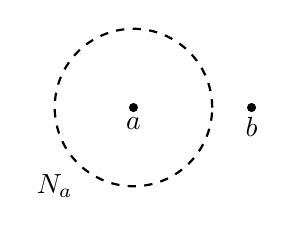
\begin{tikzpicture}
                        \draw[thick,dashed] (0,-3) circle (1cm) node (A) at (-1,-4){$N_a$};
                        \filldraw[black] (0,-3) circle (0.5mm) node[align = center, below] {$a$};
                        \filldraw[black] (1.5,-3) circle (0.5mm) node[align = center, below] {$b$};
                    \end{tikzpicture}     
                \end{center}
            \end{definition}
            \begin{definition}
                $(X,\mathcal{T})$ is said to be $\mathbf{T}_1 $ if $\forall a,b \in X$ with $a \neq b$ if $\exists N_a, N_b$ such that $b \notin N_a$ and $a \notin N_b$ 
                \begin{center}
                    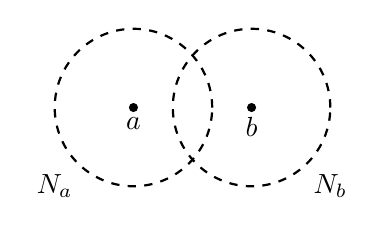
\begin{tikzpicture}
                        \draw[thick,dashed] (0,-3) circle (1cm) node (A) at (-1,-4){$N_a$};
                        \filldraw[black] (0,-3) circle (0.5mm) node[align = center, below] {$a$};
                        \draw[thick,dashed] (1.5,-3) circle (1cm) node (B) at (2.5,-4){$N_b$};
                        \filldraw[black] (1.5,-3) circle (0.5mm) node[align = center, below] {$b$};
                    \end{tikzpicture}     
                \end{center}
            \end{definition}
            \begin{definition}
                $(X,\mathcal{T})$ is said to be $\mathbf{T}_2 $ if $\exists N_a, N_b$ with $N_a \cap N_b = \varnothing$
                \begin{center}
                    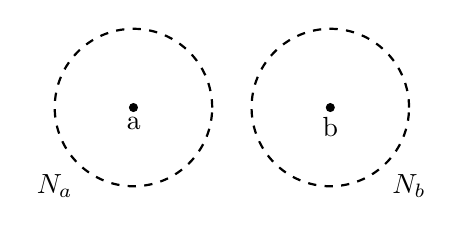
\begin{tikzpicture}
                        \draw[thick,dashed] (0,-3) circle (1cm) node (A) at (-1,-4){$N_a$};
                        \filldraw[black] (0,-3) circle (0.5mm) node[align = center, below] {a};
                        \draw[thick,dashed] (2.5,-3) circle (1cm) node (B) at (3.5,-4){$N_b$};
                        \filldraw[black] (2.5,-3) circle (0.5mm) node[align = center, below] {b};
                    \end{tikzpicture}     
                \end{center}
            \end{definition}
            \begin{obs}
                In a topological space $\mathbf{T}_2 \Rightarrow \mathbf{T}_1 \Rightarrow \mathbf{T}_0$
            \end{obs}
        \newpage
    \section*{Continous functions and homeomorphisms}
    \begin{definition}
        Let $(X, \mathcal{T}_x)$, $(\mathsf{Y}, \mathcal{T}_y)$ be topological spaces, $\varOmega : X \rightarrow \mathsf{Y}$ is continous in $a\in X$ if $\forall I $ neighbourhood of $\varOmega(a)$, $\exists K$ neighbourhood of $a$ s.t. $\varOmega(K) \subseteq I.$  
    \end{definition}
    We'll say that a function is continous if it is continous in every point.
    \begin{proposition}
        Let $\varOmega:(X, \mathcal{T}_x) \rightarrow (\mathsf{Y}, \mathcal{T}_y)$ so then the following affirmations are equivalent:
        \begin{itemize}
            \item[i.] $\varOmega$ is continous.
            \item[ii.] $\forall A \in \mathcal{T}_y,\ \varOmega^{-1}(A) \in \mathcal{T}_x.$
            \item[iii.] $\forall c \in \mathcal{C}(\mathsf{Y}), \ \varOmega^{-1}(c) \in \mathcal{C}(X).$
            \item[iv.] The counterimages of opens under a selected base of $\mathsf{Y}$ are opens of $X.$
            \item[v.] $\forall b = \varOmega(a) \in Im\varOmega = \varOmega(X)$ the counterimage  of every neighbourhood $K'$ of $b$ is a neighbourhood of $a$      
        \end{itemize}
        \begin{proof}
            $i. \Rightarrow ii.$ \ Let $A \in \mathcal{T}_y$ we have to prove that $\forall a \in \varOmega^{-1}(A)$ exists a neighbourhood of $a$ contained in $\varOmega^{-1}(A).$ For $a \in \varOmega^{-1}(A)$ one has $\varOmega(a) \in \varOmega(\varOmega^{-1}(A)) = A.\ A$ is open and is a neighbourhood of $\varOmega(a)$ so if $\varOmega$ is continous there exists a neighbourhood $K$ of $a$ s.t. 
            $\varOmega(K) \subseteq A$ hence $K \subseteq \varOmega^{-1}(A)$ and $a \in K.$ \\
            $ii. \Rightarrow i.$ Let $a \in X, \ I$ neighbourhood of $\varOmega(a)$ let $A \in \mathcal{T}_y$ s.t. $\varOmega(a) \in A \subseteq K$ for the $ii.$ $\varOmega^{-1}(A)$ is open and is a neighbourhood of $a$ s.t. its image contains $\varOmega(a)$ and $A$ is contained in $I$.
        \end{proof}
    \end{proposition}
    
\end{document}